\chapter{Experimental Setup}

In this chapter, we describe the experimental setup and the design choices made in adapting and building our agent scaffold upon existing frameworks, and the specific procedures for evaluating the proposed inference-time scaling (ITS) strategies. The primary objective is to establish a replicable evaluation framework that can quantitatively assess the impact of these ITS techniques when applied to open-source Large Language Models (LLMs) in complex machine learning engineering tasks.

To achieve this, we first describe the main components of our experimental environment: the AI-Driven Exploration (AIDE) agent scaffold, which forms the basis for our agent development, and the MLE-Bench benchmark, which provides the tasks for evaluation. We then elaborate on the significant engineering efforts undertaken to adapt these tools for effective use with locally hosted open-source LLMs, including the development of a custom vLLM-based backend for AIDE and a parallelized execution environment for MLE-Bench experiments. Finally, we outline the chosen baseline models, the specific subset of MLE-Bench competitions used, the evaluation metrics, and the overall experimental pipeline designed to ensure fair comparisons.

\section{AIDE: AI-Driven Exploration in the Code Space}
AIDE is an open source agent scaffold, developed by WecoAi (Schmidt et al., 2025). It is specifically designed to automate the trial and error process in developing machine learning models, working iteratively to find a solution in a tree search manner, exploring the `Code space`. 

The core principle behind AIDE is to address the significant amount of time that engineers and scientists spend on iterative experimentation, rather than to focus on conceptualizing and innovating.  To achieve that, AIDE frames the entire machine learning engineering process as a code optimization problem, modeling the trial and error as a tree search within a space of potential code solutions, each node is a potential solution problem (i.e. a code script), and each edge is an attempt at improving/debugging that solution. figure \ref{fig:aide-solution-tree} shows a sample solution tree for AIDE.

\begin{figure}[htbp]
    \centering
    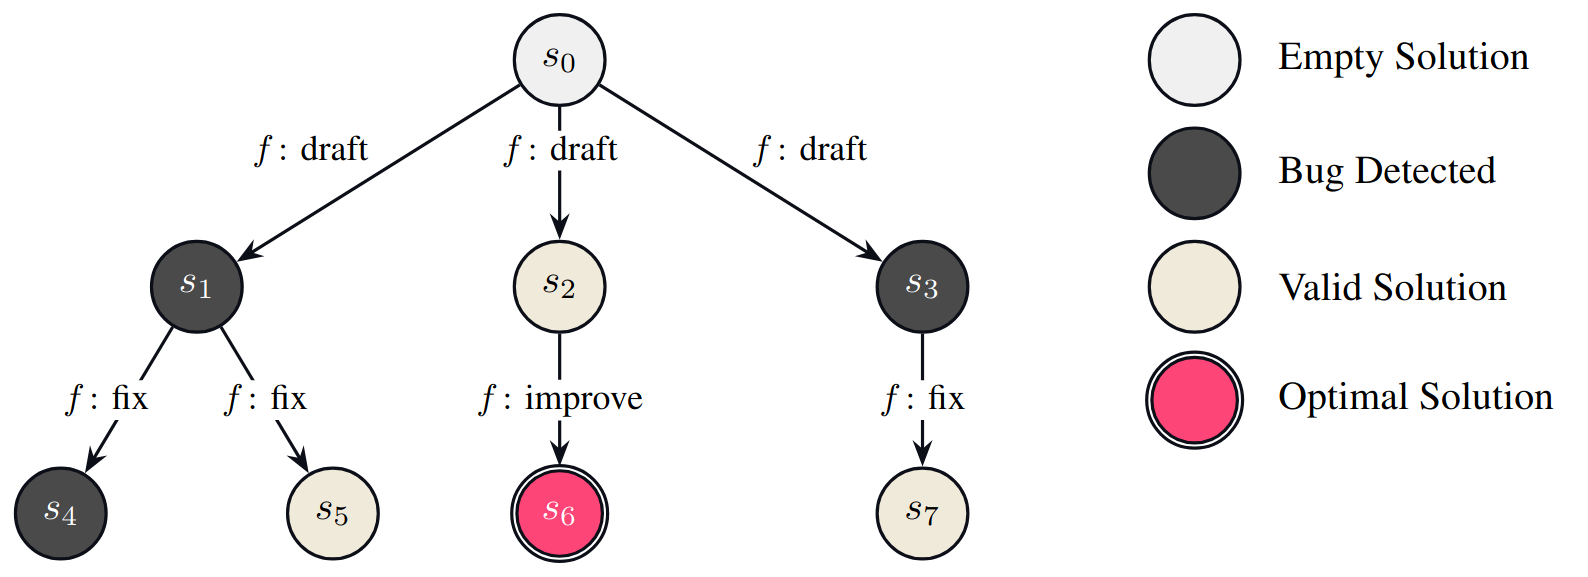
\includegraphics[width=0.8\linewidth]{images/aide-solution-tree.png}
    \caption{A sample solution tree for AIDE, illustrating the drafting, debugging, and improvement steps. (Source: Schmidt et al., 2025, p. 4)}
    \label{fig:aide-solution-tree}
\end{figure}

At its heart. and as many other agent scaffolds, AIDE is powered by a Large Language Model, typically a strong model like gpt4 or Claude. These LLMs are responsible for proposing new code, debugging existing scripts, or suggesting and improvement or refinement to promising solutions. AIDE then reuses and refines these solutions, effectively trading computational resources for improved performance. Essentially, AIDE is performing some sort of inference time scaling, as it create an iterative loop of drafting, debugging and improving code solutions but the scope and the level of this scaling is not as intensive. The implementation of AIDE is publicly available, which is why we chose it for this thesis, allowing integration of custom inference time scaling methods.

\subsection{Core Components and Methodology of AIDE}
Below is a breakdown of how AIDE operates as outlined in their original paper(Schmidt et al).

The Solution Tree ($T$): This is all discovered/proposed solutions (Python code scripts) and the improvement attempts (edges linking them) stored in a tree structure. The root solution ($s_0$) is typically an empty script, a node with value 'None'. The tree is used to store the history of the search process. In code this is typically saves as a Journal file (json) which documents the entire search process.

Evaluator ($h$): This is a stateless function that takes a solution script as input and returns a scalar score (e.g., validation accuracy, loss). This score guides the search process. this evaluator is composed of a code interpreter that executes the code, then another LLM then takes the execution result (the traceback) and produces a structured output via function calling. this particular role is considered stateless since it always produce the same score, and it does not include past attempts in its evaluation, and this is important in the overall tree search for the best solution as every node or possible solution is evaluated primary on this.

Search Policy ($\pi$): AIDE uses a simple, hard-coded search policy that determines the next step or next action. Based on the current state of the solution tree, it decides to:

1. Draft a new initial solution (if a desired number of diverse starting points hasn't been reached).
At the beginning of the search, AIDE will draft a number of initial solution that will represent an initial exploration of the solution space, this is done by prompting the LLM to generate a plan to solve the problem and then generate a single-file self contained Python program implementing that plan. These are then separated using regular expressions. The llm is also given a data preview of the dataset, and a set of instructions describing the desired output format and the metric to be used for evaluation.

In the drafting phase, AIDE asks the llm to generate a simple solution, without any optimization or hyperparameter tuning, this is done to ensure that the solution is valid and working, and to get a baseline score to compare against. nd allow fro easy debugging and improvement.

2. Debug a buggy node (if it's within a certain debug depth).
If the draft solution is not working, AIDE will debug it by prompting the LLM to inspect the and execution traces which is reformatted into a structured output, and then generate a plan to fix the script and the updated solution is then evaluated.
The debug is controlled by a probability parameter, and the default is set to 1, meaning that 100\% of the time, AIDE will debug if there is something to debug, although this can be changed to a lower value to encourage more exploration and avoid getting stuck in a local optimum.

3. Improve an existing, non-buggy solution (typically targeting the current best-performing one).
In the improvement phase, AIDE will prompt the LLM to propose a single `atomic` change, such as switching an optimizer or adding a regularization technique, so its impact on performance can be directly measured. AIDE will keep asking for improvements until the time limit is reached, or the maximum number of steps is reached.

Coding Operator or coder model ($F$): This is the LLM itself as it proposes new scripts. It has three main entry points described in the search policy, Drafting, Debugging and Improving, each with specialized prompts. these coding agents are facilitated using modular backend script for each model provider like Openai, Anthropic, Google, or Meta. and the switch between them is done using a dispatcher logic that routes the request to the appropriate model provider based on the model id.

Data Preview in Coding Prompts: AIDE also includes a small, static `data preview' in its coding prompts, providing the LLM with basic knowledge of the dataset's size or feature layout without needing extensive exploratory data analysis (EDA) at each step. As there is a code interpreter part of this iterative process, this Data preview tells the model exactly where and how the data is organized, and where to save its output or `submission.csv`

Finally, to manage the LLM's context window and avoid `prompt explosion' from an  the growing history being fed to the model during the debugging and improvement phases, AIDE uses a summarization operator. Instead of appending all historical logs, this operator selectively extracts relevant information from the solution tree, such as Performance metrics (accuracy, AUC-ROC, etc.), Hyperparameter settings from previous attempts, Relevant hints for debugging (e.g., misaligned array shapes from trace-backs), This concise summary allows each code revision to be somewhat stateless yet guided by prior information, maintaining efficiency.

The choice of AIDE as the foundational scaffold for this research is deliberate. It is open-source , it allows for the modification and integration of the inference-time scaling methods (self-consistency and self-reflection, etc) that are central to our work. Furthermore, AIDE's design, which explicitly models ML engineering as an iterative code optimization and tree search process powered by an LLM, provides a structured environment to study the effects of these techniques. It is established and proven to work effectively in solving ML tasks, as demonstrated in its original paper and subsequent evaluations on benchmarks like MLE-Bench, offers a great platform for experimentation. 

AIDE has been tested and evaluated only using lagre-scale propriety LLMs, and our aim is to investigate how inference-time strategies can enhance AIDE's problem-solving capabilities, particularly its ability to make an open source, small-scale LLM generate more robust and higher-performing solutions on the challenging task like Machine learning Engineering.

A typical AIDE run usually starts by generating a draft plan and a code script implementing that plan, then the code is executed and the result is evaluated and stored as a node in the solution tree, if the code is not working, the node is marked `buggy', then the agent proceeds to the next step, queying the search policy, which first looks at the number of initial drafts, if its less than the specified number in the configuration, the decesiopn will be to draft a new solution, otherwise the search policy will look first at the good nodes, if there is any, it acts greedly and tries to improve it, if there is no good node, it decides to debug a buggy code depending on a probability parameter. The code is debugged and the process is repeated until time limit is reached, or the maximum number of steps is reached.


\section{MLE-Bench: A Benchmark for Machine Learning Engineering}

\subsection{MLE-bench Design}
The core design of MLE-Bench is mostly around its task selection. The 75 selected competitions present an extremely difficult challenge for any coding agent. As per the authors, this benchmark focuses on two design choices: i. selecting tasks that are challenging and representative of contemporary ML engineering work, and ii. being able to compare evaluation results to human-level performance.

Essentially, MLE-Bench provides an offline Kaggle competition environment. For context, Kaggle is a platform that hosts data science and ML competitions where participants build predictive models to solve real-world challenges, competing for the best score on predefined metrics and earning rankings on a leaderboard. Top performers are often awarded monetary prizes, in addition to recognition with a bronze, silver, or gold medals. MLE-Bench adopts a similar structure to Kaggle, allowing for a realistic comparison of agent performance against historical human achievements 'offline leaderboard. The final results in this benchmark are often presented in terms of the average number of medals an agent would have won, determined by comparing its solution's metric on an unseen test set against the saved leaderboard from the original Kaggle competition.

The operational scale of MLE-Bench is considerable. The total dataset size for the 75 competitions is approximately 3.3 TB, and agents are typically allowed 24 hours to attempt to solve each competition, mirroring the time pressures often found in real-world scenarios and Kaggle challenges. Furthermore, the benchmark incorporates various measures to protect against data contamination and unauthorized access to test set labels, ensuring a fair evaluation.

Each sample in MLE-bench is a Kaggle competition consisting of:
\begin{itemize}
    \item A description scraped from the "Overview" and "Data" tabs of the competition website.
    \item The competition dataset, in most cases using a new train-test split.
    \item Grading code used to evaluate submissions locally.
    \item A snapshot of the competition's leaderboard used to rank submissions against humans.
\end{itemize}

Also, the competition are annotated each with a complexity level: Low if
an experienced ML engineer can produce a sensible solution in under 2 hours excluding
the time taken to train any models, Medium if it takes between 2 and 10 hours, and High if it takes
more than 10 hours.

Finally, the benchmark has a specific grading logic for each competition based on the evaluation metric described in its original problem description. This allows local grading for submissions, with metrics varying from standard ones like Area Under the Receiver Operating Characteristic (AUROC) curve to more domain-specific loss functions. figure \ref{fig:mlebench-design} shows the conceptual design of MLE-bench
\begin{figure}
    \centering
    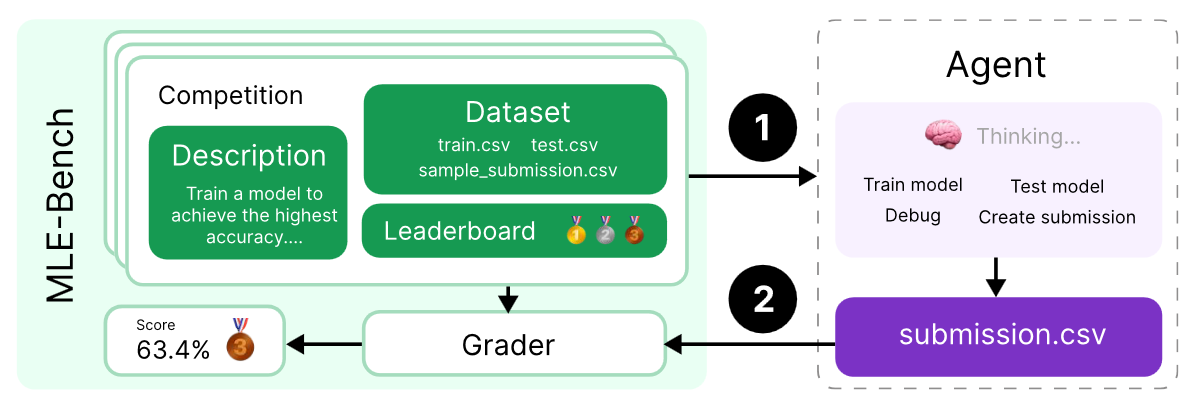
\includegraphics[width=0.75\linewidth]{images/mlebench-design.png}
    \caption{Design of MLE-bench, showing the main workflow. Source: MLE-bench~\cite{AD92}***}
    \label{fig:mlebench-design}
\end{figure}

\subsection{Key Metrics for Evaluation in MLE-Bench}
When evaluating agent performance on MLE-Bench-and our AIDE agent, several metrics are considered:
\textbf{Leaderboards}: Performance is contextualized using the private leaderboards from the original Kaggle competitions, as these are generally less prone to overfitting than public leaderboards.

\textbf{Medals}: Similar to Kaggle's system, MLE-Bench awards virtual bronze, silver, and gold medals. An agent's submission is compared against the private leaderboard of the original competition as if it were a participant at that time. The thresholds for these medals vary based on the number of teams that participated in the original competition, aiming to reflect a consistent level of achievement. 
Table \ref{tab:medal_thresholds} shows an example for medals thresholds.

\begin{table}[htbp] % htbp are placement specifiers (here, top, bottom, page)
\centering
\caption{Thresholds for winning a medal in Kaggle competitions. It varies depending on the number of teams participating in each competition. MLE-bench implements the same thresholds in the evaluation Process. Source: MLE-bench CITE HERE}
\label{tab:medal_thresholds}
\begin{tabular}{@{}l llll@{}} % @{} removes extra space at the beginning/end of table
\toprule
& \textbf{0-99 Teams} & \textbf{100-249 Teams} & \textbf{250-999 Teams} & \textbf{1000+ Teams} \\
\midrule
\textbf{Bronze} & Top 40\% & Top 40\% & Top 100 & Top 10\% \\
\textbf{Silver} & Top 20\% & Top 20\% & Top 50  & Top 5\%  \\
\textbf{Gold}   & Top 10\% & Top 10\% & Top 10  & Top 10\%  \\
\bottomrule
\end{tabular}
\end{table}

\textbf{Headline Metric}: To provide a singular, overall measure of performance, MLE-Bench reports the percentage of attempts where an agent achieved any medal (bronze or above). This is a challenging metric, designed to be comparable to the achievements of highly skilled human Kaggle participants.

\textbf{Raw Scores}: The raw score achieved by an agent on each competition's specific metric is also reported. While difficult to aggregate due to the variety of metrics, these scores are valuable for tracking competition-specific progress.

\subsection{Setup and Rules in MLE-Bench}

MLE-Bench is agnostic to the specific methods an agent uses to arrive at a solution; there is only one requirement for grading, a CSV submission file for each competition. However, when reporting results, However, special considerations should be taken when using different evaluation procedures changes (as in our case), mainly because the models, scaffolding used, internet access, hardware, runtime and whether any pre-existing solutions to the Kaggle competitions were included in the agent's prompts, can affect the performance expectation.

Core Rules:
Submissions must be generated by a model separate from the agent's core reasoning logic; the agent cannot simply write predictions to the submission file based on its own pre-trained knowledge if it has memorized labels. This ensures the agent is genuinely engaging in the ML engineering process.

Agents are prohibited from accessing external solutions online (e.g., from Kaggle or GitHub) during their run. This means that we were restricted to inference time scaling that does not involve accessing the Internet like RAG.

\subsection{Benchmark Competitions}

The foundation of our evaluation is a representative subset of competitions from the official MLE-Bench framework. While the full MLE-Bench is extensive, running experiments on all 75 competitions is computationally prohibitive for this project. Therefore, we selected a subset of 10 competitions from the 'lite' complexity category. This choice was driven by several factors:

Diversity: The selected competitions span 6 distinct machine learning categories, ensuring that our evaluation is not biased towards a single problem type. This diversity is crucial for assessing the general applicability of the proposed inference strategies. 

Feasibility: By focusing on 'lite' competitions, which are relatively lightweight in terms of data size and complexity, our experiments can focus on the quality of the agent's problem-solving process rather than being constrained by the technical overhead of handling massive datasets.

Flexibility: The chosen set is flexible enough to be extended in future work, either by including more competitions from the 'lite' category for a full standard comparison or by adding selected 'medium' complexity tasks to further test the limits of our methods.

The 10 competitions selected for this benchmark are listed in Table \ref{tab:competitions}. and more information about them can be found in the Appendix.

\begin{table}[htbp]
\centering
\caption{Selected Benchmark Competitions from MLE-Bench 'Lite' Category}
\label{tab:competitions}
\begin{tabular}{ll}
\toprule
\textbf{Competition Name} & \textbf{Category} \\
\midrule
aerial-cactus-identification & Image Classification \\
leaf-classification & Image Classification \\
spooky-author-identification & Text Classification \\
random-acts-of-pizza & Text Classification \\
tabular-playground-series-may-2022 & Tabular \\
nomad2018-predict-transparent-conductors & Tabular \\
denoising-dirty-documents & Image to Image \\
text-normalization-challenge-english-language & Sequence to Sequence \\
text-normalization-challenge-russian-language & Sequence to Sequence \\
mlsp-2013-birds & Audio Classification \\ \hline
\end{tabular}
\end{table}

\subsection{Baselines for Comparison}

To properly contextualize the performance of our proposed methods, we will benchmark them against a diverse set of established baselines. The aim is to first prove that our strategies provide a meaningful improvement over a standard open-source model, and second, to demonstrate that these strategies make open-source models competitive with both closed-source counterparts and human experts.

The baselines are summarized in Table \ref{tab:baselines}.

\begin{table}[htbp]
\centering
\caption{Baselines for Performance Comparison}
\label{tab:baselines}
\begin{tabular}{p{4cm} l p{6.5cm}}
\toprule
\textbf{Baseline} & \textbf{Type} & \textbf{Reason for Inclusion} \\
\midrule
\textbf{AIDE + GPT-4o} & CS / High-Capability & Represents a strong, widely-used frontier model. Provides a high-water mark for performance. \\
\textbf{AIDE + o4-mini} & CS / Reasoning-Optimized & Assumed to be a cost-effective, state-of-the-art reasoning model from OpenAI. Serves as a key SOTA reference. \\
\textbf{Our Model + Default AIDE} & OS / Ablation & \textbf{Critical baseline.} This isolates the performance gain attributable specifically to our inference strategies, by removing them from our chosen model. \\
\textbf{Human Performance} & Human Eval & Provides real-world context by comparing agent scores to the original Kaggle leaderboards. \\
\bottomrule
\end{tabular}
\end{table}

% 3. Evaluation Metrics

% To capture a holistic view of agent performance, we will use a suite of metrics inspired directly by the MLE-Bench and AIDE papers. These metrics evaluate an agent's ability to produce functional code, understand the task requirements, and ultimately generate an optimal solution.

% Code and Submission Generation: These metrics assess the fundamental ability of the agent to generate working code and complete the task.

% Valid Code Rate (\%): The number of steps that produce a valid, executable script divided by the total number of steps, averaged across seeds and competitions. A higher rate indicates a stronger fundamental code generation capability.

% Valid Submission Rate (\%): The percentage of independent runs (i.e., per seed, per competition) that successfully produce a submission file that passes the benchmark's validity checks. This is a stricter measure of task completion.

% Performance Against Human Baselines: Once a valid submission is produced, its quality is scored against the historical human leaderboard.

% Above Median (\%): The percentage of competitions where the agent's best score is strictly better than the median score achieved by human participants.

% Any Medal (\%): The percentage of competitions where the agent's best score is high enough to have earned a bronze, silver, or gold medal according to official Kaggle rules. This is our headline metric for overall success.

% The final results for each agent configuration will be presented in a summary table, as shown in the template in Table \ref{tab:results_template}.

% % \begin{table}[h!]
% % \centering
% % \caption{Template for Aggregated Results Table}
% % \label{tab:results_template}
% % \begin{tabular}{lccc}
% % \hline
% % \textbf{Model + Method} & \textbf{Valid Submission (\%)} & \textbf{Above Median (\%)} & \textbf{Any Medal (\%)} \ \hline
% % AIDE + o4-mini & X% 
% % ±
% % ±
% %  Y & X% 
% % ±
% % ±
% %  Y & X% 
% % ±
% % ±
% %  Y \
% % Our Model + Strategy 1 & X% 
% % ±
% % ±
% %  Y & X% 
% % ±
% % ±
% %  Y & X% 
% % ±
% % ±
% %  Y \
% % Our Model + Default AIDE & X% 
% % ±
% % ±
% %  Y & X% 
% % ±
% % ±
% %  Y & X% 
% % ±
% % ±
% %  Y \ \hline
% % \end{tabular}
% % \end{table}

\subsection{Experimental Procedure}

To ensure a fair and repeatable evaluation, all experiments are conducted using a standardized protocol within a consistent environment.

\textbf{Environment}: unless otherwise specified, all runs are executed within a Dockerized environment to ensure consistency. AIDE is configured with fixed hyperparameters for all methods (e.g., 20 steps per attempt, 5 initial drafts).

\textbf{Execution}: For each of the 10 competitions, every agent configuration ("Method") is run for k=6 independent attempts (seeds). This helps account for the inherent stochasticity of LLMs.

\textbf{Data Collection}: After each run, we automatically collect the raw data, including whether a valid submission was generated and its corresponding score using wandb[CITATION].

\textbf{Metric Calculation}: Using the collected data, we calculate the flags for Valid Submission, Above Median, and Any Medal for each run.

\textbf{Aggregation}: These flags are then aggregated. For metrics like Above Median and Any Medal, we consider a competition "solved" if at least one of the k seeds was successful (a pass@k approach). The final percentages are averaged across the 10 competitions, with results reported as mean ± standard error.

This standardized pipeline ensures that as we introduce and test new inference-time strategies, the results are directly and fairly comparable to our established baselines.


\subsection{Adapting AIDE for Local LLM Serving}

The first major technical change was to modify AIDE's backend to support locally hosted open-source LLMs, moving away from its default reliance on external API calls to proprietary models. as the original design contained backend logic for OpenAI, Google, Anthropic, and Meta.

The primary goal was to enable AIDE to utilize models from the Hugging Face ecosystem, served locally using any open source LLM inference engine like Ollama, Hugging Face Text Generation Inference (TGI), or vLLM.

\textbf{Initial Ollama Integration}: The first iteration focused on integrating with Ollama. This inference engine was chosen for its ease of setup and friendly user interface, as it automatically serves models via an API endpoint that is largely compatible with OpenAI's API specifications. The existing OpenAI backend within AIDE was adapted to redirect API calls to the local Ollama server endpoint (\textbf{http://localhost:11434/v1/}) and adjusting error handling to be compatible with Ollama's responses rather than OpenAI's specific error types. The API key field was repurposed (set to 'ollama') as authentication is handled differently for local models.

\textbf{Function Calling Challenge}: A significant challenge emerged related to AIDE's two-model pipeline:

Coding Model: The main model and coding operator responsible for generating Python code fro every phase of the AIDE process (intended to be a DeepSeek model).

Feedback Model: Evaluates the output of the executed code and ideally returns structured feedback (a JSON object indicating success/failure, metrics, and a summary) using a mechanism often referred to as "function calling" or "tool use." This is the model's primsry role is to reformat the excution output into a structured output that can be used to save and compare the results and build the tree reliably, and also to aviod expoloding context window from the error traceback.

After the Ollama integration, preliminary model testing yielded several key observations:

\textbf{Function Calling Instability}: The primary bottleneck was the unreliability of structured output generation (function calling) from the open-source models tested via Ollama for the feedback mechanism. This often led to the AIDE pipeline breaking.
Models like (deepseek-coder base, deepseek-r1-tool-calling:1.5b-7b), either did not reliably support the precise structured output format required by AIDE's feedback loop or produced outputs that led to pipeline instability. And Attempts to use models like Mistral-7B and Llama3.2 as the feedback model also encountered similar issues.

\textbf{Limited Control}: The level of control over model loading parameters (precision, specific quantization methods) and inference settings was insufficient for the experimentation with ITS strategies.

\textbf{Performance Discrepancies (Initial DeepSeek Tests on House Prices)}:

Using OpenAI's o3-mini as the feedback model (due to its reliable function calling) and a locally served DeepSeek model (via Ollama) as the coding model, stark differences were observed on a very simple task like the "house prices prediction" dataset (a common Kaggle getting-started competition, not part of the full MLE-Bench suite at this stage but used for quicker iteration).

Both DeepSeek variants,7B and 14b that were served via Ollama struggled significantly, often failing to produce a valid submission within 25 iterations, indicating issues with its ability to debug or refine its own code effectively in this setup. And the DeepSeek-32B variant was extremely slow and failed to produce a submission. A crucial later discovery was that Ollama, by default for many models (especially those tagged :latest), serves quantized versions. This was not immediately apparent and led to an underestimation of the models' true capabilities in early tests, consuming valuable time with sub-optimal model representations. This experience underscored the importance of meticulous control over model loading and precision.

This issue, and the fact that Ollama does not support many models that are available in the Hugging Face ecosystem, led to the decision to switch to a more reliable inference engine.


\textbf{Transition to Hugging Face transformers for Enhanced Control}:
To address these limitations and gain more explicit control, the AIDE backend was first refactored to directly leverage Hugging Face's transformers library, specifically using the AutoModelForCausalLM interface. This shift provided several advantages:

\textbf{Direct Model Parameter Access}: It allowed for precise control over loading models in full precision (e.g., bfloat16) or specific quantization types (8-bit via bitsandbytes), which was crucial for fair evaluation and understanding the impact of model fidelity.

\textbf{Granular Inference Control}: Direct use of the library enabled fine-tuning of generation parameters (temperature, top-p, top-k, etc.) essential for implementing ITS techniques like self-consistency.

\textbf{Improved Output Consistency}: While function calling remained a challenge for some base models, the direct interaction generally led to more predictable and sensible outputs from the models during initial testing with the 7B (full precision) and 14B (8-bit quantized) DeepSeek variants.

\subsection{vLLM Integration}

\textbf{vLLM} (\url{https://github.com/vllm-project/vllm}) stands for virtual large language models, is a high-throughput, memory-efficient library for Large Language Model (LLM) inference and serving. It's designed to make LLM deployment easier and faster, especially for production-scale applications. vLLM utilizes techniques like PagedAttention and continuous batching to optimize memory usage and improve serving throughput.

\textbf{Optimizing for Throughput and Parallelism}:
While the direct Hugging Face transformers integration offered control, running multiple experiments or even single AIDE runs (which involve numerous LLM calls) was still time-consuming due to the overhead of loading and running models sequentially for each call or experiment. To enable efficient parallel experimentation and high-throughput inference necessary for evaluating ITS strategies across multiple seeds and competitions, the backend was further evolved to integrate with vLLM.

\textbf{vLLM Backend Design}: A new backend component was developed for AIDE. This component makes API calls to a locally hosted vLLM server endpoint, which serves the desired open-source model (DeepSeek 7B, 14B, or 32B).

\textbf{Significant Throughput Improvement}: vLLM's architecture, optimized for batched inference and efficient memory management, substantially reduced the inference time. For instance, a standard 25-step AIDE run, which could take around 2 hours using Hugging Face, was reduced to under an hour for baseline models, even with multiple concurrent calls.

\textbf{Enabling Parallel Experimentation}: This vLLM-based setup has become the cornerstone for the experimental evaluation. It allowed for running multiple AIDE runs (different seeds or different ITS strategies) to concurrently query the same deployed LLM instance, with vLLM handling the parallel request serving. This was initially managed via separate bash scripts (using the apmersand \& operator) orchestrating multiple AIDE processes, each pointing to the same vLLM endpoint.

how the backedn was modified, 
then how the mlebench was modified
then the specefication of the setup hardware and software
then the 


